\section{How to choose $\epsilon$} %%%%%%%%%%%%%%%%%%%%%%%%%%%%%%%%%%%%%%%%%%%%%%%%%%%%%%%%%%%%%%%%%%%%%%%%%%%%%%%%%%%%%
This section will look at how the different projection methods compare to each other in relation to error, energy and time consumption. There will also be a comparison between restart variable and computation time. 

%\subsection{}


\subsection{Constant energy} \label{sec:SLMconstant}%%%%%%%%%%%%%%%%%%%%%%%%%%%%%%%%%%%%%%%%%%%%%%%%%%%%%%%%%%%%%%%%%%
!!!!!!!!!!!!!!!!!!!!!Det må skrives en del mer i dette kapitelet!!!!!!!!!!!!!!!!!!!!!!\\

\begin{figure}[H]
        \centering
        
		\begin{subfigure}[b]{0.3\textwidth}
                \includegraphics[width=\textwidth]{../MATLAB/fig/compareEnergyw.jpg}
                \caption{ Energy. }
                \label{fig:compareEnergyw}
        \end{subfigure}
        ~
        \begin{subfigure}[b]{0.3\textwidth}
                \includegraphics[width=\textwidth]{../MATLAB/fig/compareErrorw.jpg}
                \caption{ Error. }
                \label{fig:compareErrorw}
        \end{subfigure}
        ~
        \begin{subfigure}[b]{0.3\textwidth}
                \includegraphics[width=\textwidth]{../MATLAB/fig/compareIterw.jpg}
                \caption{ Number of restarts.  }
                \label{fig:compareIterw}
        \end{subfigure}
        
        \begin{subfigure}[b]{0.3\textwidth}
                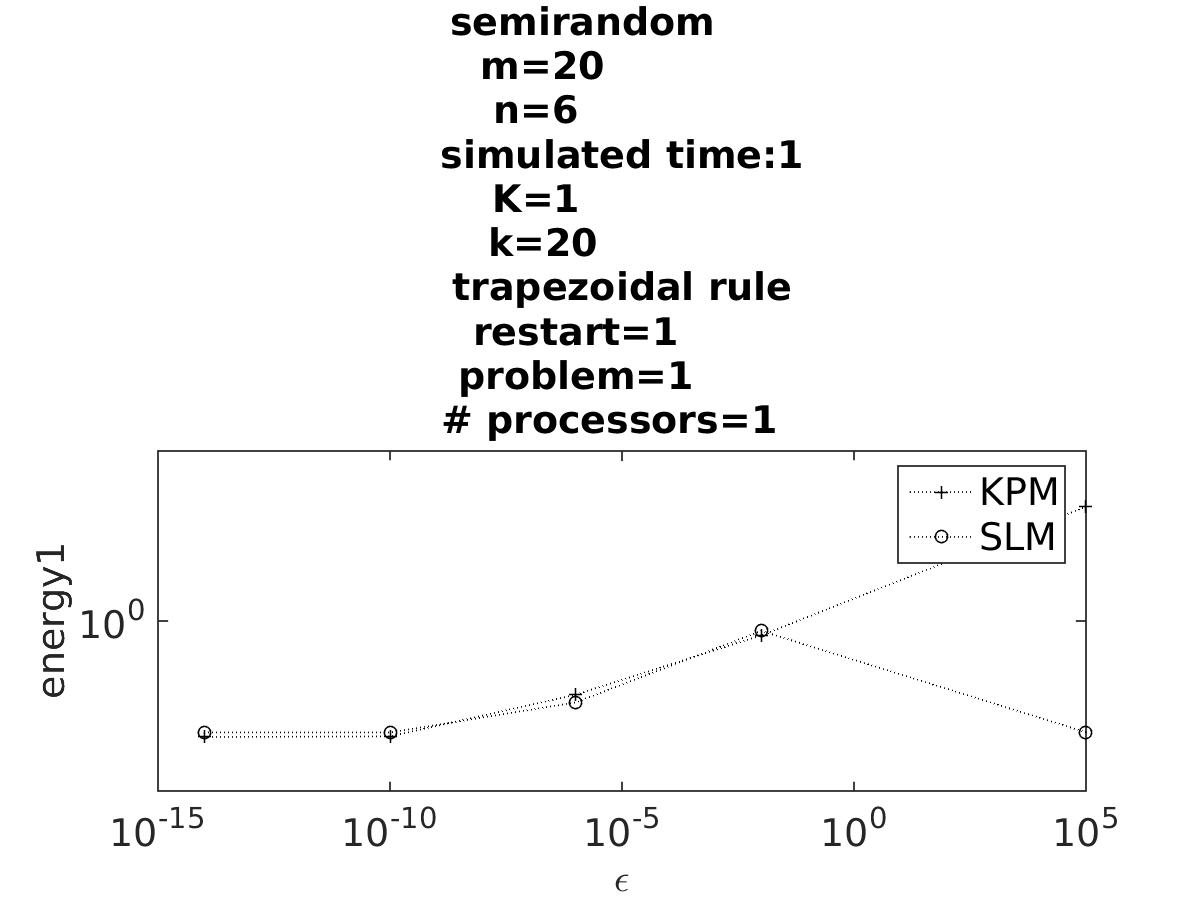
\includegraphics[width=\textwidth]{../MATLAB/fig/compareEnergy.jpg}
                \caption{Energy.}
                \label{fig:compareEnergy}
        \end{subfigure}
        ~
        \begin{subfigure}[b]{0.3\textwidth}
                \includegraphics[width=\textwidth]{../MATLAB/fig/compareError.jpg}
                \caption{ Error. }
                \label{fig:compareError}
        \end{subfigure}
        ~
        \begin{subfigure}[b]{0.3\textwidth}
                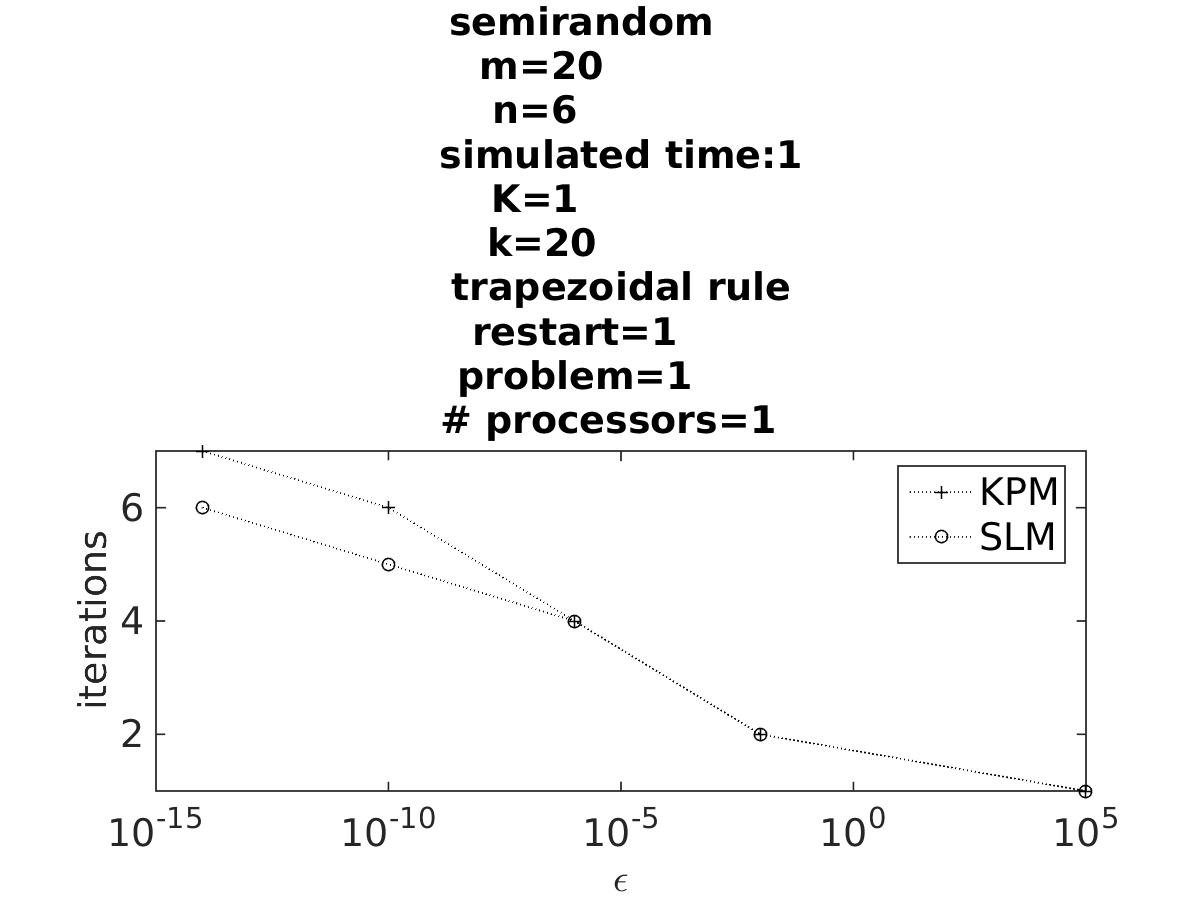
\includegraphics[width=\textwidth]{../MATLAB/fig/compareIter.jpg}
                \caption{ Number of restarts.  }
                \label{fig:compareIter}
        \end{subfigure}
        \caption{ The figure shows how the different methods change the energy and error with different number of restart for \texttt{semirandom}.  }
        \label{fig:compare}
\end{figure}



There is a clear difference between how well the energy is estimated for \texttt{wave} and \texttt{semirandom}. For \texttt{semirandom} there is not much difference between SLM and Arnoldi, although SLM seams to give a slight better approximation than Arnoldi. With \texttt{semirandom} at $\epsilon = 10^{-10}$ Arnoldi preforms one more iteration than SLM, which makes it give a better approximation, aside from that SLM consistently preform better than Arnoldi.\\
When comparing figure \ref{fig:compare} and figure \ref{fig:comparew} it is important to remember that the way the $er_1$ and $er_2$ is found is very differently, and that might explain the why the cases differs so much. But the difference might also be explained with \texttt{semiradom} being a much harder equation to solve.\\
!!!!!!!!!!!!!Skriv litt mer om hvorfor bildene for semirandom og wave er så forksjelkige!!!!!!!!!!!!!!!!!!!!!\\

\subsection{Varying energy}%%%%%%%%%%%%%%%%%%%%%%%%%%%%%%%%%%%%%%%%%%%%%%%%%%%%%%%%%%%%%%%%%%%%%%%%%%%%%%%%%%%%%%%%%%%


\begin{figure}[H]
        \centering
        
        \begin{subfigure}[b]{0.3\textwidth}
                \includegraphics[width=\textwidth]{../MATLAB/fig/compareEnergy2w.jpg}
                \caption{ The difference in energy with and without restart. }
                \label{fig:compareEnergy2w}
        \end{subfigure}
        ~
        \begin{subfigure}[b]{0.3\textwidth}
                \includegraphics[width=\textwidth]{../MATLAB/fig/compareError2w.jpg}
                \caption{ The difference in energy with and without restart. }
                \label{fig:compareError2w}
        \end{subfigure}
        ~
        \begin{subfigure}[b]{0.3\textwidth}
                \includegraphics[width=\textwidth]{../MATLAB/fig/compareIter2w.jpg}
                \caption{ The number of iterations performed with and without restarting.  }
                \label{fig:compareIter2w}
        \end{subfigure}
        
        \begin{subfigure}[b]{0.3\textwidth}
                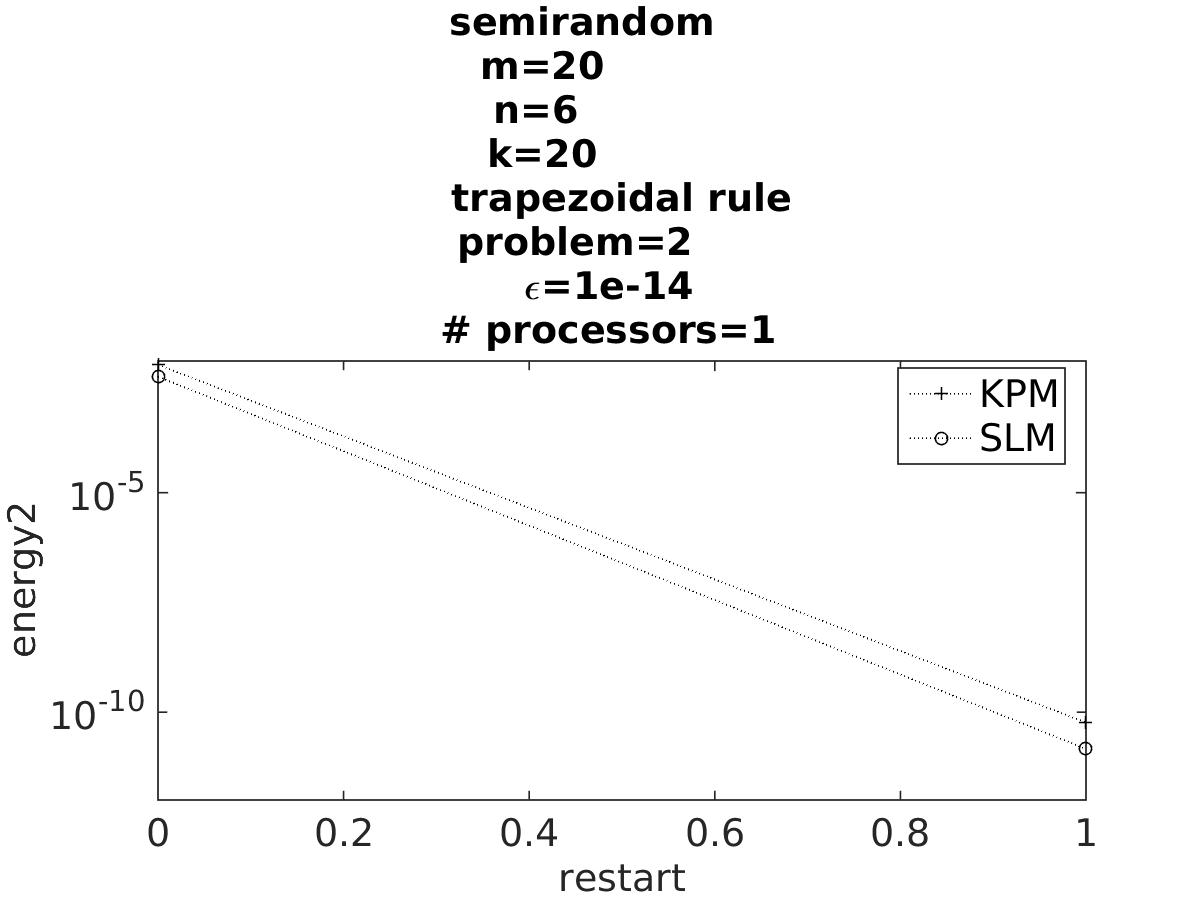
\includegraphics[width=\textwidth]{../MATLAB/fig/compareEnergy2.jpg}
                \caption{ The difference in energy with and without restart. }
                \label{fig:compareEnergy2}
        \end{subfigure}
        ~
        \begin{subfigure}[b]{0.3\textwidth}
                \includegraphics[width=\textwidth]{../MATLAB/fig/compareError2.jpg}
                \caption{ The difference in energy with and without restart. }
                \label{fig:compareError2}
        \end{subfigure}
        ~
        \begin{subfigure}[b]{0.3\textwidth}
                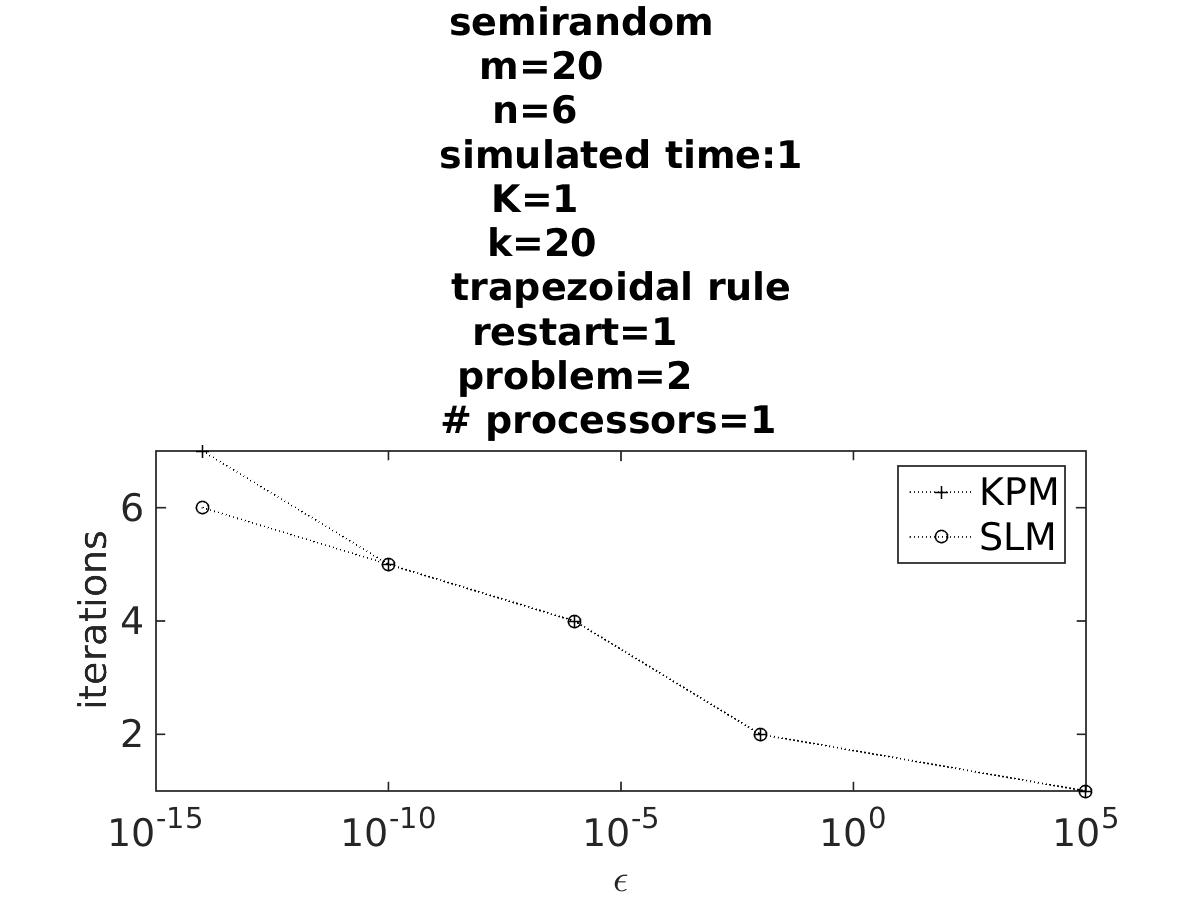
\includegraphics[width=\textwidth]{../MATLAB/fig/compareIter2.jpg}
                \caption{ The number of iterations performed with and without restarting.  }
                \label{fig:compareIter2}
        \end{subfigure}
        \caption{ The figure shows how the different methods change the energy and error with different number of restart for \texttt{wave}.  }
        \label{fig:compare2}
\end{figure}


The results here are very similar to the results found in section \ref{sec:SLMconstant}, except that the energy and error changes for the first points for both SLM and Arnoldi. SLM still gives the better approximation.

\subsection{A rule based for $\epsilon$}

\begin{figure}[H]
        \centering
        
        \begin{subfigure}[b]{0.3\textwidth}
                \includegraphics[width=\textwidth]{../MATLAB/fig/ruleerr.jpg}
                \caption{ !!!!!!!!!!!!!!!!!!!!!!!!! }
                \label{fig:ruleerr}
        \end{subfigure}
        ~
        \begin{subfigure}[b]{0.3\textwidth}
                \includegraphics[width=\textwidth]{../MATLAB/fig/ruleener.jpg}
                \caption{ !!!!!!!!!!!!!!!!!!!!!!! }
                \label{fig:ruleener}
        \end{subfigure}
        ~
        \begin{subfigure}[b]{0.3\textwidth}
                \includegraphics[width=\textwidth]{../MATLAB/fig/ruleiter.jpg}
                \caption{ !!!!!!!!!!!!!!!!!!!!  }
                \label{fig:ruleiter}
        \end{subfigure}
        
		\begin{subfigure}[b]{0.3\textwidth}
                \includegraphics[width=\textwidth]{../MATLAB/fig/ruleerr1.jpg}
                \caption{ !!!!!!!!!!!!!!!!!!!!!!!!! }
                \label{fig:ruleerr1}
        \end{subfigure}
        ~
        \begin{subfigure}[b]{0.3\textwidth}
                \includegraphics[width=\textwidth]{../MATLAB/fig/ruleener1.jpg}
                \caption{ !!!!!!!!!!!!!!!!!!!!!!! }
                \label{fig:ruleener1}
        \end{subfigure}
        ~
        \begin{subfigure}[b]{0.3\textwidth}
                \includegraphics[width=\textwidth]{../MATLAB/fig/ruleiter1.jpg}
                \caption{ !!!!!!!!!!!!!!!!!!!!  }
                \label{fig:ruleiter1}
        \end{subfigure}
        \caption{ The figure shows how the different methods change the energy and error with different number of restart for \texttt{wave}.  }
        \label{fig:rule}
\end{figure}

\section{How to choose $n$}%%%%%%%%%%%%%%%%%%%%%%%%%%%%%%%%%%%%%%%%%%%%%%%%%%%%%%%%%%%%%%%%%%%%%%%%%
The restart variable, denoted by $n$, is the size of the orthogonal system used with one of the projection method. Performing $n$ iterations of Arnoldi's algorithm or $\frac{n}{2}$ iterations of SLM gives an orthogonal space of size $n$.

\subsubsection{Constant energy}
\begin{figure}[H]
        \centering
        \begin{subfigure}[b]{0.45\textwidth}
                \includegraphics[width=\textwidth]{../MATLAB/fig/restarttime.jpg}
                \caption{  }
                \label{fig:restarttime}
        \end{subfigure}
        ~
        \begin{subfigure}[b]{0.45\textwidth}
                \includegraphics[width=\textwidth]{../MATLAB/fig/restartiter.jpg}
                \caption{  }
                \label{fig:restartiter}
        \end{subfigure}
        \begin{subfigure}[b]{0.45\textwidth}
                \includegraphics[width=\textwidth]{../MATLAB/fig/restarterror.jpg}
                \caption{  }
                \label{fig:restarterror}
        \end{subfigure}
        \begin{subfigure}[b]{0.45\textwidth}
                \includegraphics[width=\textwidth]{../MATLAB/fig/restartenergy.jpg}
                \caption{  }
                \label{fig:restartenergy}
        \end{subfigure}
        \caption{ computation time, number of restarts, error and energy are all plotted here with different $m$ and $n$. }
        \label{fig:restart}
\end{figure}

\begin{figure}[H]
        \centering
        \begin{subfigure}[b]{0.45\textwidth}
                \includegraphics[width=\textwidth]{../MATLAB/fig/restarttimeSLM.jpg}
                \caption{  }
                \label{fig:restarttimeSLM}
        \end{subfigure}
        ~
        \begin{subfigure}[b]{0.45\textwidth}
                \includegraphics[width=\textwidth]{../MATLAB/fig/restartiterSLM.jpg}
                \caption{  }
                \label{fig:restartiterSLM}
        \end{subfigure}
        \begin{subfigure}[b]{0.45\textwidth}
                \includegraphics[width=\textwidth]{../MATLAB/fig/restarterrorSLM.jpg}
                \caption{  }
                \label{fig:restarterrorSLM}
        \end{subfigure}
        \begin{subfigure}[b]{0.45\textwidth}
                \includegraphics[width=\textwidth]{../MATLAB/fig/restartenergySLM.jpg}
                \caption{  }
                \label{fig:restartenergySLM}
        \end{subfigure}
        \caption{ computation time, number of restarts, error and energy are all plotted here with different $m$ and $n$. }
        \label{fig:restartSLM}
\end{figure}
!!!!!!!!!!!!!!!Skriv noen commentarer her!!!!!!!!!!!!!!!!!!!!!!\\
\subsubsection{Varying energy}%%%%%%%%%%%%%%%%%%%%%%%%%%%%%%%%%%%%%%%%%%%%%%%%%%%%%%%%%%%%%%%%%%%%%%%%%%%%%%%%%%%%%%%%%%%
\begin{figure}[H]
        \centering
        \begin{subfigure}[b]{0.45\textwidth}
                \includegraphics[width=\textwidth]{../MATLAB/fig/restarttime2.jpg}
                \caption{  }
                \label{fig:restarttime2}
        \end{subfigure}
        ~
        \begin{subfigure}[b]{0.45\textwidth}
                \includegraphics[width=\textwidth]{../MATLAB/fig/restartiter2.jpg}
                \caption{  }
                \label{fig:restartiter2}
        \end{subfigure}
        \begin{subfigure}[b]{0.45\textwidth}
                \includegraphics[width=\textwidth]{../MATLAB/fig/restarterror2.jpg}
                \caption{  }
                \label{fig:restarterror2}
        \end{subfigure}
        \begin{subfigure}[b]{0.45\textwidth}
                \includegraphics[width=\textwidth]{../MATLAB/fig/restartenergy2.jpg}
                \caption{  }
                \label{fig:restartenergy2}
        \end{subfigure}
        \caption{ !!!!!!!!!!!!!!!!!SKRIV NOE HER!!!!!!!!!!!!!!!!!!  }
        \label{fig:restart2}
\end{figure}


!!!!!!!!!!!!!!!Kommentar her!!!!!!!!!!!!!\\
\begin{figure}[H]
        \centering
        \begin{subfigure}[b]{0.45\textwidth}
                \includegraphics[width=\textwidth]{../MATLAB/fig/restarttime2SLM.jpg}
                \caption{  }
                \label{fig:restarttime2SLM}
        \end{subfigure}
        ~
        \begin{subfigure}[b]{0.45\textwidth}
                \includegraphics[width=\textwidth]{../MATLAB/fig/restartiter2SLM.jpg}
                \caption{  }
                \label{fig:restartiter2SLM}
        \end{subfigure}
        \begin{subfigure}[b]{0.45\textwidth}
                \includegraphics[width=\textwidth]{../MATLAB/fig/restarterror2SLM.jpg}
                \caption{  }
                \label{fig:restarterror2SLM}
        \end{subfigure}
        \begin{subfigure}[b]{0.45\textwidth}
                \includegraphics[width=\textwidth]{../MATLAB/fig/restartenergy2SLM.jpg}
                \caption{  }
                \label{fig:restartenergy2SLM}
        \end{subfigure}
        \caption{ !!!!!!!!!!!!!!!!!SKRIV NOE HER!!!!!!!!!!!!!!!!!!  }
        \label{fig:restart2SLM}
\end{figure}
!!!!!!!!!!!!KOmmentar her!!!!!!!!!!!!!!!\\
figure \ref{fig:restart2} shows a few different important things. First figure \ref{fig:restarterror2} shows that the error and energy does not change (much) with $n$, only with $m$. The second thing is that the number of iterations needed to converge decreases when $n$ becomes larger. The finale thing is that there seams to be a restart variable smaller than the dimension of $A$, and larger than one that is optimal. 
!!!!!!!!!!!!KOmmentar om forskjellene på Arnoldi og SLM!!!!!!!!!!!!!!!\\

\section{Computation time}%%%%%%%%%%%%%%%%%%%%%%%%%%%%%%%%%%%%%%%%%%%%%%%%%%%%%%%%%%%%%%%%%%%%%%%%%%%%%%%%%%%%%%%%%
!!!!!!!!!!!!!!!!!!!!!!!!!!Burde jeg ha med restart eller ikke på disse bildene?!!!!!!!!!!!!!!!!!\\
!!!!!!!!!!!!!!!!!!!!!!!!!!!Begge deler sikkert!!!!!!!!!!!!!!!!!\\
!!!!!!TEXT!!!!!! \\


\subsection{Constant energy}%%%%%%%%%%%%%%%%%%%%%%%%%%%%%%%%%%%%%%%%%%%%%%%%%%%%%%%%%%%%%%%%%%%%%%%%%%%%%%%%%%%%%%%%%%
!!!!!!TEXT!!!!!! 
\begin{figure}[H]
        \centering
        \begin{subfigure}[b]{0.3\textwidth}
                \includegraphics[width=\textwidth]{../MATLAB/fig/ccomparetimem0.jpg}
                \caption{ !!!!!!TEXT!!!!!! }
                \label{fig:ccomparetimem0}
        \end{subfigure}
        ~
        \begin{subfigure}[b]{0.3\textwidth}
                \includegraphics[width=\textwidth]{../MATLAB/fig/ccomparetimem.jpg}
                \caption{ !!!!!!TEXT!!!!!! }
                \label{fig:ccomparetimem}
        \end{subfigure}
        ~

        
        \begin{subfigure}[b]{0.3\textwidth}
                \includegraphics[width=\textwidth]{../MATLAB/fig/ccomparetimek0.jpg}
                \caption{ !!!!!!TEXT!!!!!! }
                \label{fig:ccomparetimek0}
        \end{subfigure}
        ~
        \begin{subfigure}[b]{0.3\textwidth}
                \includegraphics[width=\textwidth]{../MATLAB/fig/ccomparetimek.jpg}
                \caption{ !!!!!!TEXT!!!!!! }
                \label{fig:ccomparetimek}
        \end{subfigure}
        ~

        \caption{ !!!!!!TEXT!!!!!!}
        \label{fig:ccomparetime}
\end{figure}
!!!!!!TEXT!!!!!! \\
\subsection{Varying energy}%%%%%%%%%%%%%%%%%%%%%%%%%%%%%%%%%%%%%%%%%%%%%%%%%%%%%%%%%%%%%%%%%%%%%%%%%%%%%%%%%%%%%%%%%%%
!!!!!!TEXT!!!!!! \\
\begin{figure}[H]
        \centering
        \begin{subfigure}[b]{0.3\textwidth}
                \includegraphics[width=\textwidth]{../MATLAB/fig/vcomparetimem0.jpg}
                \caption{ !!!!!!TEXT!!!!!! }
                \label{fig:vcomparetimem0}
        \end{subfigure}
        ~
        \begin{subfigure}[b]{0.3\textwidth}
                \includegraphics[width=\textwidth]{../MATLAB/fig/vcomparetimem.jpg}
                \caption{ !!!!!!TEXT!!!!!! }
                \label{fig:vcomparetimem}
        \end{subfigure}
        ~

        
        \begin{subfigure}[b]{0.3\textwidth}
                \includegraphics[width=\textwidth]{../MATLAB/fig/vcomparetimek0.jpg}
                \caption{ !!!!!!TEXT!!!!!! }
                \label{fig:vcomparetimek0}
        \end{subfigure}
        ~
        \begin{subfigure}[b]{0.3\textwidth}
                \includegraphics[width=\textwidth]{../MATLAB/fig/vcomparetimek.jpg}
                \caption{ !!!!!!TEXT!!!!!! }
                \label{fig:vcomparetimek}
        \end{subfigure}
        ~

        \caption{ !!!!!!TEXT!!!!!!}
        \label{fig:vcomparetime}
\end{figure}
!!!!!!TEXT!!!!!! \\

\subsection{Best case for SLM and KPM} %%%%%%%%%%%%%%%%%%%%%%%%%%%%%%%%%%%%%%%%%%%%%%%%%%%%%%%%%%%%%%%%%%%%%%%%%%%%%%%

\begin{figure}[H]
        \centering
        \begin{subfigure}[b]{0.3\textwidth}
                \includegraphics[width=\textwidth]{../MATLAB/fig/fastruntime1.jpg}
                \caption{ !!!!!!TEXT!!!!!! }
                \label{fig:fastruntime1}
        \end{subfigure}
        ~
        \begin{subfigure}[b]{0.3\textwidth}
                \includegraphics[width=\textwidth]{../MATLAB/fig/fastruntime3.jpg}
                \caption{ !!!!!!TEXT!!!!!! }
                \label{fig:fastruntime3}
        \end{subfigure}

        \caption{ !!!!!!TEXT!!!!!!}
        \label{fig:fastruntime}
\end{figure}
